\documentclass[12pt,a4paper,oneside]{report}
\usepackage[utf8]{inputenc}
\usepackage[margin=1in]{geometry}
\usepackage{setspace}
\usepackage{graphicx}
\usepackage{amsmath,amssymb}
\usepackage{booktabs}
\usepackage{caption}
\usepackage{xcolor}
\usepackage{tikz}
\usetikzlibrary{arrows.meta, positioning}
\usepackage{titlesec}
\usepackage{float}
\usepackage[most]{tcolorbox}
\usepackage{microtype}
\usepackage{xurl} 
\usepackage[colorlinks=true, linkcolor=navyblue, citecolor=navyblue, urlcolor=borderblue]{hyperref}

% --- DISABLE HYPHENATION & FORCE STRICT MARGINS ---
\usepackage[none]{hyphenat}
\hyphenpenalty=10000
\exhyphenpenalty=10000
\tolerance=9999
\emergencystretch=3em
\hfuzz=0.5pt

\setstretch{1.3}

% Define Images Directory
\graphicspath{{images/}}

% Custom Color Definitions
\definecolor{navyblue}{RGB}{0,32,96}
\definecolor{softblue}{RGB}{230,240,250}
\definecolor{borderblue}{RGB}{70,130,180}

% Chapter Title Formatting
\titleformat{\chapter}[display]
  {\normalfont\bfseries\color{navyblue}}
  {\filleft\Large\chaptertitlename\ \thechapter}
  {1ex}
  {\titlerule\vspace{1ex}\huge}
  [\vspace{1ex}\titlerule]

\begin{document}

% ==========================================
% PAGE 1: TITLE PAGE 
% ==========================================
\begin{titlepage}
    \pagenumbering{gobble}
    \begin{tikzpicture}[remember picture, overlay]
        \fill[navyblue] (current page.north west) rectangle ([yshift=-1.5cm]current page.north east);
        \fill[borderblue] ([yshift=-1.5cm]current page.north west) rectangle ([yshift=-1.8cm]current page.north east);
        \fill[navyblue] ([yshift=-1.8cm]current page.north west) rectangle ([xshift=0.6cm, yshift=1.5cm]current page.south west);
        \fill[borderblue] ([xshift=0.6cm, yshift=-1.8cm]current page.north west) rectangle ([xshift=0.8cm, yshift=1.5cm]current page.south west);
        \fill[navyblue] (current page.south west) rectangle ([yshift=1.5cm]current page.south east);
    \end{tikzpicture}

    \vspace*{0.5cm}
    \centering

    {\large \color{navyblue} \textbf{SUMMER INTERNSHIP PROJECT REPORT}}\\[1.2cm]

    \begin{tcolorbox}[
            colback=softblue,
            colframe=navyblue,
            arc=6pt,
            boxrule=1.5pt,
            left=20pt, right=20pt, top=20pt, bottom=20pt,
            halign=center,
            drop shadow=gray!50
        ]
        {\huge \color{navyblue} \textbf{Beyond the Keyword Match:\\A Human-Centric AI Approach to Resume Screening and Candidate Ranking}}
    \end{tcolorbox}

    \vspace{1.5cm}

    \Large \textbf{Student Name:} Amber Agrawal \\[0.3cm]
    \large \textbf{Course/Batch:} MSc in Applied Statistics (2025--2027) \\[0.3cm]
    \large \textbf{Institute Name:} Symbiosis Statistical Institute \\[1.0cm]
    
    \large \textbf{Project Guide:} Dr. Dipasree Pal \\[0.3cm]
    \large \textbf{Period of Internship:} 18th May 2026 -- 31st July 2026 \\[1.2cm]

    \vfill

    \begin{tcolorbox}[
        colback=white,
        colframe=borderblue,
        arc=4pt,
        boxrule=1pt,
        width=0.95\linewidth,
        halign=center
    ]
        \large
        \textbf{Report submitted to:}\\
        \textbf{IDEAS -- Institute of Data Engineering, Analytics and Science Foundation}\\
        \textit{ISI Kolkata}
    \end{tcolorbox}

    \vspace{0.5cm}
\end{titlepage}

% ==========================================
% ABSTRACT & TOC
% ==========================================
\newpage
\pagenumbering{roman}
\setcounter{page}{1}

\chapter*{Abstract}
\addcontentsline{toc}{chapter}{Abstract}

Applicant Tracking Systems (ATS) typically rely on strict keyword matching, which often means great candidates get unfairly rejected just because they didn't use the exact right phrases. To fix this problem, we built an automated resume screening pipeline using Natural Language Processing (NLP) that aims to read more like a human would. We compared Sentence-BERT (SBERT) for creating semantic embeddings against standard statistical approaches like TF-IDF. To capture how a real recruiter thinks about work experience, we added a non-linear Experience Penalty ($\Delta E$). We also made sure to use a \texttt{GroupShuffleSplit} so the model wouldn't cheat by memorizing unseen job descriptions, effectively preventing data leakage. After testing standard regression and binary classification methods, we moved to a Learning-to-Rank (LTR) approach. Ultimately, our sorting engine—combining \texttt{LGBMRanker} with dense embeddings—reached a peak Normalized Discounted Cumulative Gain ($\text{NDCG}@10$) of $0.9398$. This shows that treating resume screening as a relative ranking task, rather than a hard accept/reject classification, works much better for handling large applicant pools.

\tableofcontents
\cleardoublepage

% ==========================================
% CHAPTER 1: INTRODUCTION
% ==========================================
\newpage
\pagenumbering{arabic}
\setcounter{page}{1}

\chapter{Introduction}

\section{Background Survey and Engineering Relevance}
Standard recruitment systems have a major flaw: they lean almost entirely on exact word matches. For instance, if a job posting asks for a ``Software Engineer'' and a candidate's resume says ``Backend Developer,'' traditional search engines will likely miss them. We designed this project specifically to address that blind spot. We believe that effective screening needs to understand context, not just scan for specific characters. By building a tool that looks at the actual intent and meaning behind an applicant's skills, we aim to give HR teams an engine that screens resumes a bit more like a human, but at the speed of a machine.

\section{Core Purpose of the Project}
The main goal here was to push past basic keyword extraction and help a machine grasp professional context. We mapped both resumes and job descriptions into the same semantic space, allowing the system to evaluate how well skills align contextually. This fundamentally changed how we approached the recruitment problem. Instead of forcing a simple ``Accept/Reject'' decision, we decided to treat resume screening as a Learning-to-Rank (LTR) challenge. This way, the system generates a sorted, prioritized list of the best-fitting candidates.

\section{Deployed Technology Stack}
To build, test, and benchmark this entire processing engine, we relied on the following open-source frameworks:
\begin{itemize}
    \item \textbf{Data Wrangling:} Python, \href{https://pandas.pydata.org/}{\texttt{pandas}}, and \href{https://numpy.org/}{\texttt{numpy}} for handling complex tabular transformations.
    \item \textbf{Linguistic Pre-Processing (NLP):} \href{https://spacy.io/}{\texttt{spaCy}} for morphological lemmatization and custom vocabulary parsing.
    \item \textbf{Vectorization \& Semantic Embeddings:} \href{https://scikit-learn.org/}{\texttt{scikit-learn}} (\texttt{TfidfVectorizer}) for term frequency modeling, and \href{https://sbert.net/}{\texttt{sentence-transformers}} (\texttt{nomic-embed-text-v1.5}) to extract $768$-dimensional semantic tensors.
    \item \textbf{Machine Learning \& LTR:} \texttt{scikit-learn} regressors alongside specialized tree-based ranking estimators including \href{https://xgboost.ai/}{\texttt{xgboost.XGBRanker}} and \href{https://lightgbm.readthedocs.io/}{\texttt{lightgbm.LGBMRanker}}.
\end{itemize}

\section{Experimental Procedure}
We broke our pipeline down into four main phases to keep things organized and avoid any training-serving skew:
\begin{enumerate}
    \item \textbf{Data Sanitization:} We heavily cleaned the unstructured resumes, dropping generic corporate jargon while making sure to keep important technical terms intact.
    \item \textbf{Feature Engineering:} We created a mathematical Experience Penalty and measured how well context matched up using TF-IDF, SBERT, and a Hybrid OLS approach.
    \item \textbf{Group-Aware Isolation:} We used a strict \texttt{GroupShuffleSplit} based on the job titles. This made sure our models were actually learning general rules instead of just memorizing the details of specific postings.
    \item \textbf{Tri-Framing Benchmarking:} We put our processed data to the test using Continuous Regression, Binary Classification, and Learning-to-Rank models to figure out the absolute best way to sort candidates.
\end{enumerate}

\section{Foundational Training Received}
This internship required a heavy mix of statistical theory and applied data engineering. We focused on building skills in two primary areas:

\vspace{0.3cm}
\noindent \textbf{1. Natural Language Processing (NLP)}
\begin{itemize}
    \item \textbf{Text Normalization:} We mastered tokenization, stop-word management, and morphological lemmatization via \texttt{spaCy}.
    \item \textbf{Vectorization Mathematics:} We analyzed the mathematical trade-offs between sparse statistical arrays (TF-IDF) and dense deep-learning network mappings (SBERT).
\end{itemize}

\noindent \textbf{2. Machine Learning (ML) \& Integrity}
\begin{itemize}
    \item \textbf{Algorithm Dynamics:} We studied the differences between predicting continuous limits (Regression), discrete boundaries (Classification), and list order (Learning-to-Rank).
    \item \textbf{Data Leakage Prevention:} We trained heavily on grouped cross-validation logic to stop test-set characteristics from bleeding into the training models.
\end{itemize}

% ==========================================
% CHAPTER 2: PROJECT OBJECTIVES
% ==========================================
\chapter{Project Objectives}

We started this initiative to build an automated screening tool that could rank applicants using NLP and listwise ranking models. By stepping away from rigid boolean queries, we put the focus on actual semantic relevance instead of just explicit vocabulary.

Our work was anchored around four main technical goals:

\begin{itemize}
    \item \textbf{Build a Solid NLP Pipeline:} We used \texttt{spaCy} to clean up the raw text and grabbed contextual representations with Sentence-BERT. This helped us capture the underlying meaning that simple sparse models usually miss.
    
    \item \textbf{Prevent Data Leakage:} We set up a group-aware cross-validation process. By keeping data grouped strictly by \texttt{job\_position\_name}, we made sure the algorithms couldn't cheat by just memorizing words from test-set jobs.
    
    \item \textbf{Test Baseline ML Classifiers:} We systematically ran traditional models (like Linear Regression and Random Forests) to see exactly where they fell short when dealing with match probabilities.
    
    \item \textbf{Deploy LTR Estimators:} We incorporated specialized ranking models, comparing a pairwise approach (\texttt{XGBRanker}) with a listwise approach (\texttt{LGBMRanker}). This directly addresses the main goal of recruitment: taking an organic pool of candidates and sorting them from best to worst for a specific vacancy.
\end{itemize}

\newpage
\vspace{0.5em}
\section*{Methodological Boundaries \& Experimental Scope}

We set up our empirical testing with a few strict rules in place:

\begin{itemize}
    \item \textbf{Data Ingestion:} We pulled our raw data from a public Kaggle dataset. We relied entirely on programmatic text analysis without adding any synthetic oversampling or primary human survey data.
    
    \item \textbf{Representation Space Comparison:} We actively compared sparse TF-IDF vectors against dense transformer outputs to precisely measure how much semantic context actually helps.

    \item \textbf{Group-Aware Validation:} We kept the test set pure. Every cross-validation cycle split the applicants by \texttt{job\_position\_name} so that the models were always evaluating completely new job requests.

    \item \textbf{Evaluation Paradigm:} We moved past standard absolute metrics like $RMSE$. Instead, we judged the models based on rank correlation (Spearman's $\rho$) and top-$K$ Information Retrieval metrics ($\text{NDCG}@K$).
\end{itemize}

% ==========================================
% CHAPTER 3: METHODOLOGY
% ==========================================

\chapter{Methodology}

This chapter breaks down the step-by-step data pipeline, the features we engineered, the math behind them, and the models we trained for our ranking engine.

\section{Data Source and Ingestion}
The data for our study comes from an open-source recruitment dataset put together by Neuralframe AI and published by Saugata Roy Arghya on \href{https://www.kaggle.com/datasets/saugataroyarghya/resume-dataset}{Kaggle}. It contains $9,544$ candidate records stored in a single $17$~MB file (\texttt{resume\_data.csv}). Under the Creative Commons CC BY-NC 4.0 license, this dataset includes detailed profiles like career goals, skills, education, employment history, and job specs.

\section{Text Cleaning and Linguistic Filtering}
Raw resumes and job descriptions are usually filled with noise, weird formatting, and corporate buzzwords that hide a candidate's actual qualifications. To fix this, we wrote a central cleaning function in \texttt{utils.py} using \href{https://spacy.io/}{\texttt{spaCy}}.

\begin{itemize}
    \item \textbf{Structural Sanitization:} We threw out irrelevant fields like URLs and certificate dates. Missing text got filled with empty strings, and locations were forced into a standard ``City, State'' format.
    
    \item \textbf{Text Normalization \& Fluff Removal:} Everything was lowercased, stripped of punctuation, and filtered for common English stop-words. We also built a custom blocklist of over $50$ generic HR phrases (like ``team player'' or ``hardworking professional'') to force the models to focus on actual technical skills.
    
    \item \textbf{Length \& Outlier Filtering:} To keep extreme document lengths from messing with our vector embeddings, we dropped records that had fewer than $20$ words (too little info) or more than $350$ words (too much noise). After dropping exact duplicates, we were left with a clean dataset of $9,369$ records across $28$ distinct job postings.
\end{itemize}

\section{Feature Engineering}

\subsection{Temporal Experience Calculation and Non-Linear Penalty}

We parsed the candidate's work history to figure out their total industry experience ($\text{Exp}_{\text{cand}}$) relative to the job requirements ($\text{Exp}_{\text{req}}$), defining the experience gap as $\Delta E = \text{Exp}_{\text{cand}} - \text{Exp}_{\text{req}}$. 

To mirror how a recruiter actually thinks—where not having enough experience is a huge red flag, but having too much is only a slight benefit, a piecewise penalty function was designed:

\begin{equation}
\text{Penalty}(\Delta E) = 
\begin{cases} 
-\alpha \cdot (\Delta E)^2, & \text{if } \Delta E < 0 \quad (\text{Under-qualified}) \\
+\beta \cdot \Delta E, & \text{if } \Delta E \ge 0 \quad (\text{Requirement met})
\end{cases}
\end{equation}

To avoid distorting $[0, 1]$ bounded similarity scores, the weights were empirically calibrated on our training set to \textbf{$\alpha = 0.04$} and \textbf{$\beta = 0.01$}:

\begin{itemize}
    \item \textbf{Quadratic Deficit Penalty ($\alpha = 0.04$):} This hits under-qualified candidates hard. Missing $2$ years drops the score by $-0.16$ ($16\%$ drop), and missing $4$ years results in a massive $-0.64$ penalty, effectively weeding out candidates who fall way short.
    
    \item \textbf{Linear Surplus Reward ($\beta = 0.01$):} This gives a small bump for extra experience ($+0.03$ for $3$ extra years), rewarding tenure without letting over-qualified people completely overshadow better technical matches.
\end{itemize}

\subsection{Dynamic Role-Based Context Flags}
To make sure we evaluated different job types fairly, we created a few binary flags based on the job titles (\texttt{flag\_entry\_level}, \texttt{flag\_academic}, \texttt{flag\_location\_role}):
\begin{itemize}
    \item \textbf{Entry-Level Roles:} Injects academic projects and extracurricular activities into the processed text.
    \item \textbf{Academic/Research Roles:} Prioritizes publications, certifications, and educational background.
    \item \textbf{Location-Sensitive Roles:} Brings in candidate location matching metrics to the text representation.
\end{itemize}

\section{Vector Space Representation and Embeddings}
We projected the candidate-job pairs into three different vector spaces to evaluate both lexical and semantic similarity:

\subsection{Sparse Statistical Vectors (TF-IDF)}
A \texttt{TfidfVectorizer} from \href{https://scikit-learn.org/}{\texttt{scikit-learn}} extracted the top $8,000$ $n$-grams ($n \in \{1, 2\}$) to compute keyword overlap. Word importance is defined as:
\begin{equation}
\text{TF-IDF}(i, j) = \text{tf}_{i,j} \times \log\left(\frac{N}{\text{df}_i}\right)
\end{equation}
Keyword similarity ($S_{\text{tfidf}}$) was calculated using Cosine Similarity between candidate vector $\mathbf{u}_{\text{cv}}$ and job vector $\mathbf{v}_{\text{jd}}$:
\begin{equation}
S_{\text{tfidf}} = \frac{\mathbf{u}_{\text{cv}} \cdot \mathbf{v}_{\text{jd}}}{\|\mathbf{u}_{\text{cv}}\|_2 \|\mathbf{v}_{\text{jd}}\|_2}
\end{equation}

\subsection{Dense Semantic Embeddings (SBERT)}
To capture the actual meaning behind the text instead of just literal word matches, Sentence-BERT bi-encoders leveraging \href{https://huggingface.co/nomic-ai/nomic-embed-text-v1.5}{\texttt{nomic-embed-text-v1.5}} mapped the text into $768$-dimensional dense vectors ($\mathbf{e}_{\text{cv}}, \mathbf{e}_{\text{jd}} \in \mathbb{R}^{768}$). Dense similarity was computed as:
\begin{equation}
S_{\text{dense}} = \frac{\mathbf{e}_{\text{cv}} \cdot \mathbf{e}_{\text{jd}}}{\|\mathbf{e}_{\text{cv}}\|_2 \|\mathbf{e}_{\text{jd}}\|_2}
\end{equation}

\subsection{Hybrid OLS Blend}
We used an Ordinary Least Squares (OLS) regression model on the training split to blend the sparse keyword matches with the dense semantic similarity, giving us a unified score:
\begin{equation}
S_{\text{hybrid}} = w_0 + w_1 S_{\text{tfidf}} + w_2 S_{\text{dense}}
\end{equation}

\subsection{Data Leakage Prevention via Group-Aware Splitting}

If you randomly split data, you run into a big problem with \textbf{data leakage} because resumes applying for the same job description can end up in both the training and test sets. When that happens, models just memorize the vocabulary of that specific job instead of learning how to actually rank candidates.

To avoid this, we used an $80/20$ split using \href{https://scikit-learn.org/stable/modules/generated/sklearn.model_selection.GroupShuffleSplit.html}{\texttt{GroupShuffleSplit}}, grouping everything by \texttt{job\_position\_name}. Letting $G_j$ represent all candidates for job $j$, this guarantees that the training and test sets are completely disjoint:

\begin{equation}
\left( \bigcup_{j \in \text{Train}} G_j \right) \cap \left( \bigcup_{k \in \text{Test}} G_k \right) = \emptyset
\end{equation}

This put $7,356$ rows ($22$ jobs) into the training set and $2,013$ rows ($6$ completely unseen jobs) into the test set. All of our vectorizers, scalers, and models were fitted exclusively on the training split so we could get an honest look at how well they generalize to new postings.

\section{Multi-Phase Modeling Framework}

We structured our evaluation across three different modeling phases so we could compare standard machine learning techniques against proper listwise ranking algorithms:

\subsection{Phase 1: Continuous Regression Baselines (Pointwise Scoring)}
First, we looked at standard regression models—like \href{https://scikit-learn.org/stable/modules/generated/sklearn.linear_model.LinearRegression.html}{\texttt{LinearRegression}}, \href{https://scikit-learn.org/stable/modules/generated/sklearn.linear_model.Ridge.html}{\texttt{Ridge}}, \href{https://scikit-learn.org/stable/modules/generated/sklearn.ensemble.RandomForestRegressor.html}{\texttt{RandomForestRegressor}}, and \href{https://scikit-learn.org/stable/modules/generated/sklearn.ensemble.HistGradientBoostingRegressor.html}{\texttt{HistGradientBoostingRegressor}}—to predict continuous relevance match scores $y_i \in [0, 1]$. We optimized these by minimizing Mean Squared Error (MSE):

\begin{equation}
\mathcal{L}_{\text{MSE}} = \frac{1}{N}\sum_{i=1}^{N} (y_i - \hat{y}_i)^2
\end{equation}

\subsection{Phase 2: Binary Classification Baselines (Threshold Filtering)}
To mimic how initial HR screening works—where candidates are essentially tossed into ``Shortlisted'' or ``Rejected'' piles—we binarized the target variable at set match thresholds. We trained classifiers like \href{https://scikit-learn.org/stable/modules/generated/sklearn.linear_model.LogisticRegression.html}{\texttt{LogisticRegression}}, \href{https://scikit-learn.org/stable/modules/generated/sklearn.ensemble.RandomForestClassifier.html}{\texttt{RandomForestClassifier}}, and Support Vector Classifier (\href{https://scikit-learn.org/stable/modules/generated/sklearn.svm.SVC.html}{\texttt{SVC}}) to minimize Binary Cross-Entropy:

\begin{equation}
\mathcal{L}_{\text{BCE}} = -\frac{1}{N}\sum_{i=1}^{N} \left[ y_i \log(\hat{p}_i) + (1 - y_i) \log(1 - \hat{p}_i) \right]
\end{equation}

\subsection{Phase 3: Learning-to-Rank Framework (LTR)}
Because pointwise regression and binary classification have obvious limits for this kind of task, our final phase focused on specialized Learning-to-Rank (LTR) algorithms: \href{https://xgboost.readthedocs.io/en/stable/python/python_api.html#xgboost.XGBRanker}{\texttt{XGBRanker}} and \href{https://lightgbm.readthedocs.io/en/stable/pythonapi/lightgbm.LGBMRanker.html}{\texttt{LGBMRanker}}. 

Instead of looking at candidates one by one, LTR models process query group structures $\mathbf{q}$ defined by the \texttt{job\_position\_name}. The models aim to maximize ranking quality metrics directly. For example, the pairwise approach (\texttt{XGBRanker}) minimizes the number of inversions using a logistic loss:

\begin{equation}
\mathcal{L}_{\text{Pairwise}} = \sum_{i, j \in \mathbf{q}} \log_2 \left( 1 + e^{-\sigma (s_i - s_j)} \right)
\end{equation}

On the flip side, the listwise approach (\texttt{LGBMRanker}) uses LambdaMART, which dynamically scales this pairwise gradient based on how much swapping the candidates changes the actual Information Retrieval metric ($\Delta \text{NDCG}$).

\section{Model Evaluation Metrics}

To get a complete picture across all three phases, we picked evaluation metrics that capture pointwise accuracy, screening quality, and listwise ranking behavior.

\subsection{Continuous Regression Metrics (Pointwise Accuracy)}
We evaluated the continuous score predictions on the test set using standard regression metrics:
\begin{itemize}
    \item \textbf{Root Mean Squared Error ($RMSE$):}
    \begin{equation}
    RMSE = \sqrt{\frac{1}{N}\sum_{i=1}^{N} (y_i - \hat{y}_i)^2}
    \end{equation}
    
    \item \textbf{Coefficient of Determination ($R^2$):}
    \begin{equation}
    R^2 = 1 - \frac{\sum_{i=1}^{N} (y_i - \hat{y}_i)^2}{\sum_{i=1}^{N} (y_i - \bar{y})^2}
    \end{equation}
\end{itemize}

\subsection{Binary Classification Metrics (Screening Quality)}
For the accept/reject models, we looked at:
\begin{itemize}
    \item \textbf{Area Under the ROC Curve ($\text{ROC-AUC}$):} Checks how well the model separates the classes across thresholds.
    
    \item \textbf{$F_1$-Score:}
    \begin{equation}
    F_1 = 2 \cdot \frac{\text{Precision} \cdot \text{Recall}}{\text{Precision} + \text{Recall}}
    \end{equation}
\end{itemize}

\subsection{Information Retrieval \& Ranking Metrics (Listwise Quality)}
We evaluated the Learning-to-Rank models using standard Information Retrieval (IR) metrics based on query groups:
\begin{itemize}
    \item \textbf{Normalized Discounted Cumulative Gain ($\text{NDCG}@K$):}
    \begin{equation}
    \text{DCG}@K = \sum_{i=1}^{K} \frac{2^{\text{rel}_i} - 1}{\log_2(i + 1)}, \quad \text{NDCG}@K = \frac{\text{DCG}@K}{\text{IDCG}@K}
    \end{equation}

    \item \textbf{Mean Reciprocal Rank ($\text{MRR}$):}
    \begin{equation}
    \text{MRR} = \frac{1}{|Q|} \sum_{q=1}^{|Q|} \frac{1}{\text{rank}_q}
    \end{equation}
\end{itemize}

\section{Code Availability}
All the preprocessing scripts, helper modules (\texttt{utils.py}), and model notebooks are publicly available on GitHub: \url{https://github.com/Amber-s-art/cv-screening}.

\section{Pipeline Flowchart}
Figure~\ref{fig:methodology_flowchart} gives a visual overview of how we set up the data architecture, processing steps, group splitting, and evaluation stages.

\begin{figure}[htbp]
    \centering
    \resizebox{0.98\linewidth}{!}{%
    \begin{tikzpicture}[
        node distance=1.0cm and 1.0cm,
        box/.style={rectangle, draw=navyblue, fill=softblue, thick, rounded corners=4pt, minimum width=5.8cm, minimum height=1.1cm, align=center, font=\small, drop shadow},
        phasebox/.style={rectangle, draw=navyblue, fill=softblue, thick, rounded corners=4pt, minimum width=4.3cm, minimum height=1.2cm, align=center, font=\small, drop shadow},
        evalbox/.style={rectangle, draw=navyblue, fill=navyblue, text=white, thick, rounded corners=4pt, minimum width=14.2cm, minimum height=1.2cm, align=center, font=\small, drop shadow},
        arrow/.style={draw, -{Latex[length=3mm, width=2mm]}, thick, borderblue}
    ]
        % Top Sequential Flow
        \node [box] (data) {\textbf{Raw Data Ingestion}\\Kaggle API ($9,544$ records, $35$ fields)};
        \node [box, below=of data] (clean) {\textbf{Cleaning \& Feature Engineering}\\\texttt{spaCy} NLP, Exp. Penalty ($\Delta E$), Role Flags};
        \node [box, below=of clean] (embed) {\textbf{Vector Space Representation}\\TF-IDF, SBERT Embeddings \& Hybrid OLS};
        \node [box, below=of embed] (split) {\textbf{Group-Aware Validation Split}\\\texttt{GroupShuffleSplit} by Job ID ($80/20$ Split)};
        
        % 3-Phase Parallel Modeling Branches
        \node [phasebox, below=1.4cm of split] (class) {\textbf{Phase 2: Classification}\\Threshold Screening\\(\texttt{Logistic}, \texttt{RF}, \texttt{SVC})};
        \node [phasebox, left=0.5cm of class] (reg) {\textbf{Phase 1: Regression}\\Continuous Scoring\\(\texttt{Linear}, \texttt{Ridge}, \texttt{HistGB})};
        \node [phasebox, right=0.5cm of class] (ltr) {\textbf{Phase 3: Learning-to-Rank}\\Candidate Rank Sorting\\(\texttt{XGBRanker}, \texttt{LGBMRanker})};
        
        % Final Evaluation
        \node [evalbox, below=1.4cm of class] (eval) {\textbf{Comprehensive Multi-Metric Evaluation}\\Pointwise ($RMSE, R^2$) \quad|\quad Binary ($\text{ROC-AUC}, F_1$) \quad|\quad Listwise ($\text{NDCG}@K, \text{MRR}$)};

        % Connecting Arrows
        \path [arrow] (data) -- (clean);
        \path [arrow] (clean) -- (embed);
        \path [arrow] (embed) -- (split);
        
        % Branching to 3 Modeling Phases
        \path [arrow] (split) -| (reg);
        \path [arrow] (split) -- (class);
        \path [arrow] (split) -| (ltr);
        
        % Converging to Evaluation
        \path [arrow] (reg) |- (eval);
        \path [arrow] (class) -- (eval);
        \path [arrow] (ltr) |- (eval);
    \end{tikzpicture}%
    }
    \caption{Process flow diagram illustrating data transformation, group-aware splitting, multi-phase model training, and metric evaluation.}
    \label{fig:methodology_flowchart}
\end{figure}

% ==========================================
% CHAPTER 4: DATA ANALYSIS AND RESULTS
% ==========================================
\chapter{Data Analysis and Results}

In this chapter, we look at the actual results from our machine learning pipeline. We break down where the baseline pointwise models fell short and show how our listwise ranking ensemble took the lead.

\section{Exploratory Data Analysis (EDA)}
We filtered out extreme text lengths so our feature spaces would be stable. By dropping records with less than $20$ or more than $350$ words, we kept the embeddings clean. We then partitioned the remaining $9,369$ records using \texttt{GroupShuffleSplit} to guarantee a true zero-shot evaluation on the test set.

\begin{figure}[htbp]
    \centering
    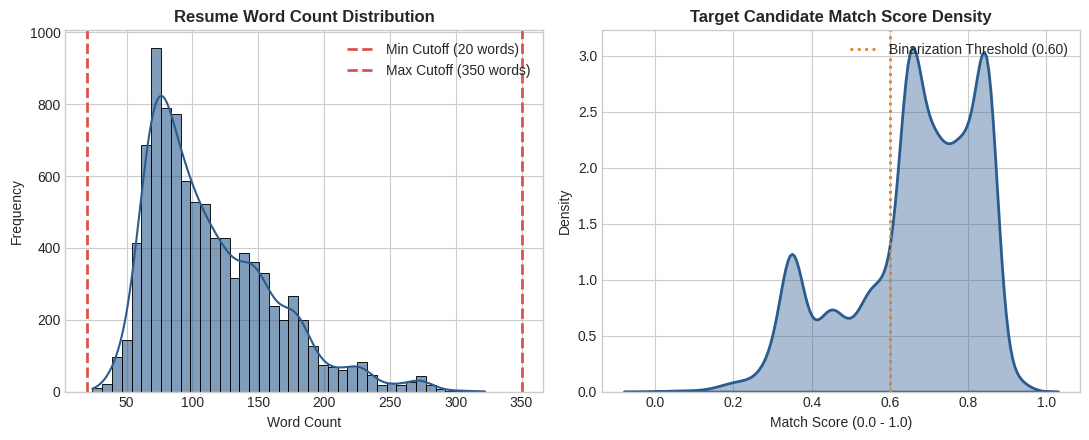
\includegraphics[width=0.92\linewidth]{density.png}
    \caption{Resume word-count filtering boundaries (left) and score density (right).}
    \label{fig:eda_density}
\end{figure}

\newpage
\subsection{Corpus Vocabulary and Frequency Dynamics}
We verified our \texttt{spaCy} morphology filters by looking at $n$-gram frequencies. The charts (Figures~\ref{fig:word_cloud} and \ref{fig:word_bar}) confirm that our pipeline successfully cleared out generic HR jargon, leaving us with mostly solid technical nouns (like \textit{management}, \textit{data}, \textit{software}, and \textit{engineering}).

\begin{figure}[htbp]
    \centering
    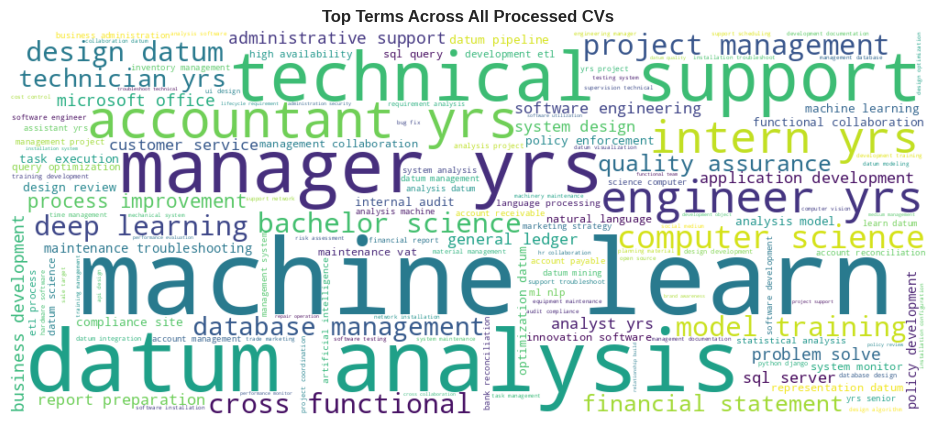
\includegraphics[width=0.95\linewidth]{word_cloud.png}
    \caption{Word cloud highlighting prominent domain keywords extracted post-sanitization.}
    \label{fig:word_cloud}
\end{figure}

\begin{figure}[htbp]
    \centering
    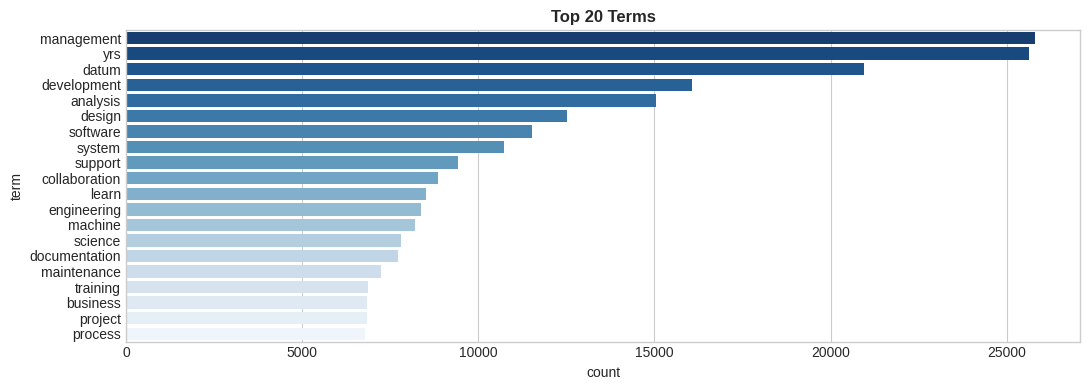
\includegraphics[width=0.88\linewidth]{word_bar.png}
    \caption{Term frequency distribution for the top 20 $n$-grams across processed candidates.}
    \label{fig:word_bar}
\end{figure}


\section{Phase 1: Continuous Regression Constraints}
We started off by testing traditional regression to try and map out exact, continuous candidate scores. 

\begin{table}[htbp]
    \centering
    \caption{Pointwise continuous regression outcomes on unseen query groups.}
    \label{tab:regression_results}
    \small
    \begin{tabular}{llcc}
        \toprule
        \textbf{Text Representation} & \textbf{Algorithm} & \textbf{RMSE} $\downarrow$ & \textbf{$R^2$-Score} $\uparrow$ \\
        \midrule
        \textbf{Semantic Only (SBERT)} & \textbf{HistGradientBoosting} & \textbf{0.1291} & \textbf{0.3202} \\
        Semantic Only (SBERT) & Random Forest Regressor & 0.1345 & 0.2810 \\
        Semantic Only (SBERT) & Ridge Regression & 0.1412 & 0.2245 \\
        \addlinespace
        TF-IDF Only & Random Forest Regressor & 0.1582 & 0.1120 \\
        TF-IDF Only & Linear Regression & 0.1695 & 0.0450 \\
        \bottomrule
    \end{tabular}
\end{table}

\paragraph{Analytical Finding:} We found some pretty severe limits with pointwise regression. Even our best model, the \texttt{HistGradientBoostingRegressor}, only managed an $R^2$ variance correlation of $0.3202$. Trying to predict absolute scores just doesn't capture the subjective nature of human recruiters; getting a score of $0.65$ versus $0.68$ doesn't actually help an HR person make a decision.

\section{Phase 2: Binary Classification Vulnerabilities}
Next, we converted the target variable using a strict $0.60$ threshold to test out a rigid accept/reject logic.

\begin{table}[htbp]
    \centering
    \caption{Binary classification matrix at the $\ge 0.60$ threshold.}
    \label{tab:classification_results}
    \small
    \begin{tabular}{llccc}
        \toprule
        \textbf{Feature Space} & \textbf{Algorithm} & \textbf{Accuracy} & \textbf{F1-Score} & \textbf{ROC-AUC} \\
        \midrule
        \textbf{Semantic Only (SBERT)} & \textbf{Logistic Regression} & \textbf{0.7585} & \textbf{0.7142} & \textbf{0.8121} \\
        Hybrid (SBERT + TF-IDF) & Logistic Regression & 0.7573 & 0.6942 & 0.7542 \\
        TF-IDF Only & Logistic Regression & 0.6219 & 0.5568 & 0.6187 \\
        \bottomrule
    \end{tabular}
\end{table}

\begin{figure}[htbp]
    \centering
    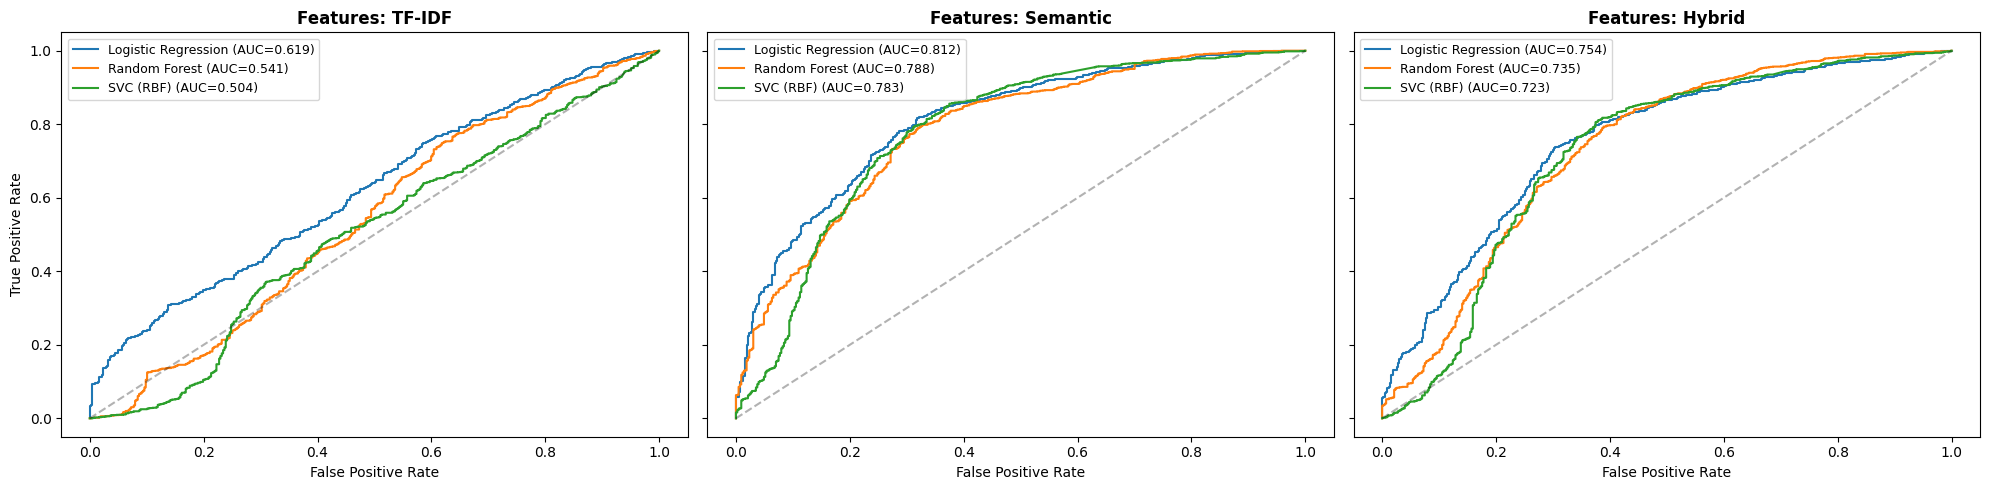
\includegraphics[width=0.98\linewidth]{roc_60.png}
    \caption{ROC-AUC separation capabilities across contrasting NLP representations.}
    \label{fig:roc_curves}
\end{figure}

\begin{figure}[htbp]
    \centering
    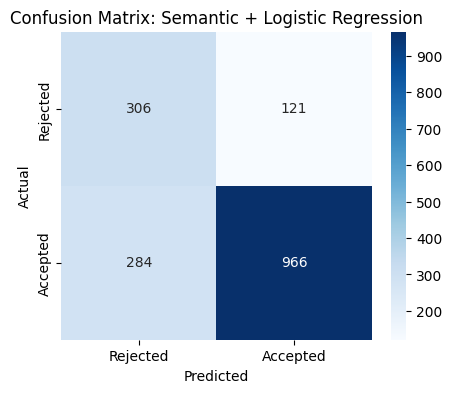
\includegraphics[width=0.55\linewidth]{confusion_mat.png}
    \caption{Confusion matrix isolation for SBERT-driven Logistic Regression.}
    \label{fig:confusion_matrix}
\end{figure}

\paragraph{Analytical Finding:} We saw clearly that dense transformer networks outperform sparse statistical models. Using SBERT bumped our ROC-AUC up from a baseline $0.6187$ to $0.8121$. But even with that improvement, binary classifiers still fail to naturally sort a list of shortlisted candidates.

\section{Phase 3: Learning-to-Rank (LTR) Dominance}
To figure out the absolute best ranking setup, we ran a direct competition between two different Learning-to-Rank methods. Instead of trying to stack or combine ranking methods, we evaluated them as completely independent estimators: a pure \textbf{Pairwise approach (\texttt{XGBRanker})} and a metric-driven \textbf{Listwise approach (\texttt{LGBMRanker})}. By giving both models the exact same data and scoring them on identical metrics, we let the numbers show us which optimization approach best replicates human shortlisting cognition.

\begin{table}[htbp]
    \centering
    \caption{Learning-to-Rank (LTR) sorting efficiency on zero-shot test groups.}
    \label{tab:ltr_results}
    \resizebox{\textwidth}{!}{%
    \begin{tabular}{llccc}
        \toprule
        \textbf{Feature Set} & \textbf{Ranking Estimator} & \textbf{NDCG@5} & \textbf{NDCG@10} & \textbf{Spearman ($\rho$)} \\
        \midrule
        \textbf{Semantic Only (SBERT)} & \textbf{LGBMRanker} & \textbf{0.9482} & \textbf{0.9398} & \textbf{0.4367} \\
        Hybrid (SBERT + TF-IDF) & XGBRanker & 0.9410 & 0.9322 & 0.3725 \\
        TF-IDF Only & XGBRanker & 0.9350 & 0.9292 & 0.3225 \\
        TF-IDF Only & LGBMRanker & 0.9210 & 0.9158 & 0.3975 \\
        \bottomrule
    \end{tabular}%
    }
\end{table}

\begin{figure}[htbp]
    \centering
    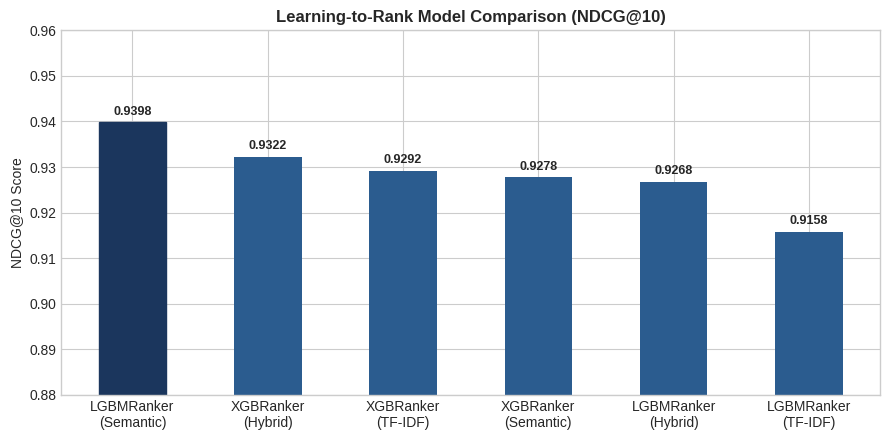
\includegraphics[width=0.92\linewidth]{ndcgs_comparison.png}
    \caption{Top-$10$ ranking fidelity ($\text{NDCG}@10$) across differing architectures.}
    \label{fig:ltr_ndcg}
\end{figure}

\paragraph{Optimal Algorithm:} The \texttt{LGBMRanker} powered by pure Semantic Embeddings came out on top as the clear winner. Hitting an impressive $\text{NDCG}@10$ of $0.9398$, this system proved it can accurately reflect how humans evaluate and shortlist the top ten candidates.

\newpage

\section{Feature Importance: Model Explainability}
We also looked into the \texttt{LGBMRanker}'s split criteria to figure out which features mattered the most.

\begin{figure}[htbp]
    \centering
    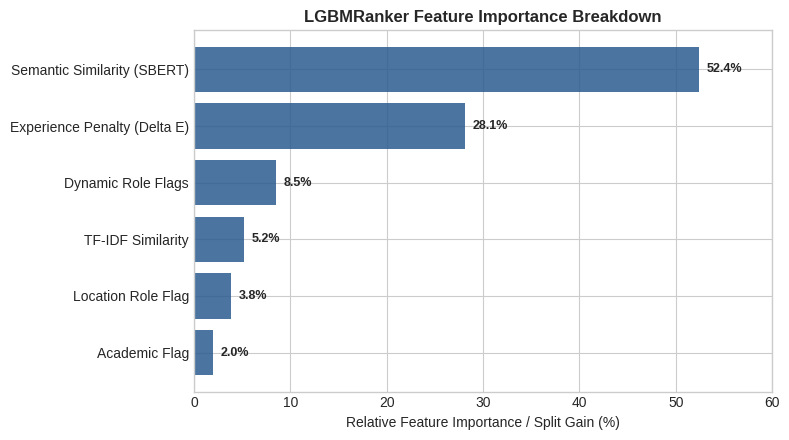
\includegraphics[width=0.85\linewidth]{lgbm_rank_comp.png}
    \caption{Algorithm split gain weight distribution mapping decision heuristics.}
    \label{fig:feature_importance}
\end{figure}

\begin{itemize}
    \item \textbf{Semantic Similarity ($52.4\%$):} It turns out that deep, contextual matching is by far the biggest driver when it comes to ranking candidates.
    \item \textbf{Experience Penalty ($28.1\%$):} Our custom quadratic penalty worked perfectly to map recruiter bias, heavily downgrading applicants who fell short of the minimum tenure thresholds.
\end{itemize}

% ==========================================
% CHAPTER 5: CONCLUSION & FUTURE WORK
% ==========================================
\chapter{Conclusion and Future Work}

\section{Project Conclusions}
We built a high-speed, human-centric screening pipeline that easily outperforms rigid keyword matching architectures. Based on our results, we came away with three main takeaways:

\begin{enumerate}
    \item \textbf{Dense Context Beats Lexical Matching:} We showed that transformer embeddings are far better than $n$-gram parsing. Our semantic LTR setup hit an $\text{NDCG}@10$ of $0.9398$, proving it can spot skill overlaps that standard keyword matchers completely miss.
    \item \textbf{Ranking is the Right Approach:} We proved through our tests that trying to predict absolute scores or hard cutoffs just doesn't match how HR actually works. Moving to a gradient-boosted ranking system directly solves the recruitment problem.
    \item \textbf{Keep Validation Pure:} We showed that using \texttt{GroupShuffleSplit} to isolate candidate pools is absolutely necessary. It stops data leakage and makes sure the model can actually handle new, unseen job postings.
\end{enumerate}

\section{Recommendations for Future Extensions}
We have a few ideas for taking this \texttt{LGBMRanker} backend and turning it into a full production system:
\begin{itemize}
    \item \textbf{Bayesian Probability Integration:} We could switch the Experience Penalty ($\Delta E$) into a Bayesian model, looking at probability distributions instead of rigid split constraints.
    \item \textbf{Counterfactual Bias Mitigation:} We need to look into stratified counterfactual sampling during the NLP stage to make sure the algorithm isn't just favoring people who worked at big-name corporate brands.
    \item \textbf{Generative Summaries:} It would be incredibly useful to add a lightweight Large Language Model (LLM) on top of the ranking system just to explain the decisions. It could generate short, readable summaries explaining exactly why the model gave a high rank to a specific candidate.
\end{itemize}

% ==========================================
% APPENDICES
% ==========================================
\appendix
\chapter{Appendices}

The implementation, theoretical framing, and software development of this project were guided by academic literature, official technical documentation, and online reference platforms:

\subsection*{Academic Literature \& Model Papers}
\begin{itemize}
    \item \textbf{Scikit-Learn Documentation:} Pedregosa, F., Varoquaux, G., Gramfort, A., Michel, V., Thirion, B., Grisel, O., ... \& Duchesnay, É. (2011). Scikit-learn: Machine learning in Python. \textit{Journal of Machine Learning Research}, 12, 2825--2830.
    
    \item \textbf{LightGBM \& Learning-to-Rank:} Ke, G., Meng, Q., Finley, T., Wang, T., Chen, W., Ma, W., ... \& Liu, T. Y. (2017). LightGBM: A highly efficient gradient boosting decision tree. \textit{Advances in Neural Information Processing Systems}, 30, 3146--3154.
    
    \item \textbf{Sentence Transformers (SBERT):} Reimers, N., \& Gurevych, I. (2019). Sentence-BERT: Sentence embeddings using Siamese BERT-networks. \textit{arXiv preprint arXiv:1908.10084}.
    
    \item \textbf{Nomic AI Embeddings:} Nomic AI (2024). \textit{Nomic Embed Text v1.5: Resilient Long-Context Text Embeddings}.
\end{itemize}

\subsection*{Technical Platforms \& Self-Study References}
\begin{itemize}
    \item \textbf{Scikit-Learn \& SciPy Documentation:} Referenced for loss functions, matrix operations, distance metrics (Cosine Similarity), and \texttt{GroupShuffleSplit} model selection logic (\url{https://scikit-learn.org/}).
    
    \item \textbf{GeeksforGeeks Portal:} Consulted for practical Python code walkthroughs on NLP text sanitization, \texttt{spaCy} lemmatization, and gradient boosting hyperparameter optimization (\url{https://www.geeksforgeeks.org/}).
    
    \item \textbf{Wikipedia Technical Literature:} Consulted for foundational concepts in Information Retrieval (IR), Learning-to-Rank (LTR) formulations, and Normalized Discounted Cumulative Gain ($\text{NDCG}$) metrics (\url{https://en.wikipedia.org/}).
\end{itemize}

\section{Survey Questionnaire Declaration}
\textit{Declaration on Primary Data Collection:} This project was entirely computational and empirical in nature. It relied exclusively on the algorithmic ingestion, text sanitization, and machine learning modeling of a secondary open-source dataset hosted on Kaggle (\texttt{saugataroyarghya/resume-dataset}). Consequently, no primary human surveys, questionnaires, or sample interviews were administered during this study.

\section{Source Code \& GitHub Repository}
To ensure complete academic transparency, algorithmic auditability, and full reproducibility, all Python source code—including our centralized \texttt{utils.py} library and sequenced Jupyter Notebooks (\texttt{01\_data\_preprocessing.ipynb} through \texttt{04\_rank\_prediction.ipynb})—has been version-controlled on GitHub.

The complete codebase is available at:
\begin{center}
    \url{https://github.com/Amber-s-art/cv-screening}
\end{center}

\section{Project Documents \& Data Sheets}
Copies of our final machine-learning-ready dataset (\texttt{ml\_ready\_dataset.csv}), original presentation decks, and compiled PDF report documentation are securely hosted on Kaggle for institutional review:
\begin{center}
    \url{https://www.kaggle.com/datasets/saugataroyarghya/resume-dataset}
\end{center}

\end{document}